\chapter{Geometria/Números (4º Bimestre)}

\section{Corpos redondos}

\subsection*{Retas e segmentos}

A circunferência de um círculo é o conjunto de todos os pontos do plano
que são equidistantes ao centro.

\begin{center}
 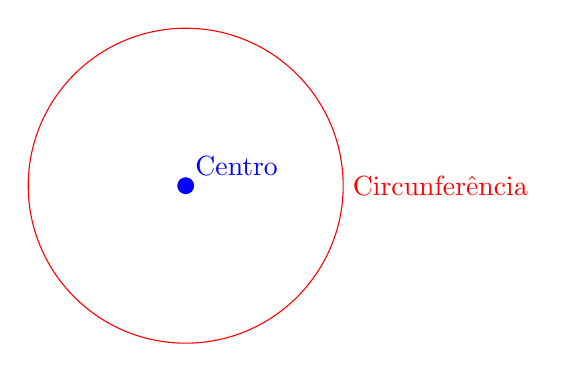
\begin{tikzpicture}
   \draw[color=blue] (0,0) node[above right]{Centro} circle(.1)[fill=blue];
   \draw[color=red] (0,0)  circle(2) (2,0) node[right] {Circunferência};
 \end{tikzpicture}
\end{center}

O raio é o segmento une o centro a um ponto da circunferência.

\begin{center}
 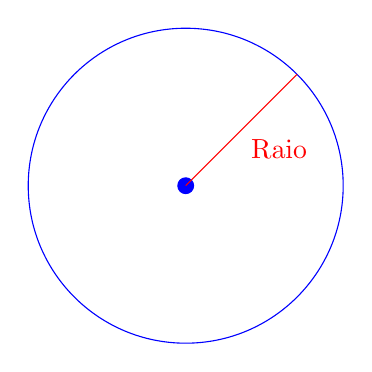
\begin{tikzpicture}
   \draw[color=blue] (0,0) circle(.1)[fill=blue];
   \draw (0,0)  circle(2)[color=blue];
   \draw[color=red]
   (0,0) -- (0.70710678118654,0.70710678118654)node[below right]{Raio} --
   (1.414213562373095,1.414213562373095);
 \end{tikzpicture}
\end{center}

O diâmetro é um segmento que une dois pontos da circunferência
e que passa pelo centro. Se $R$ é o comprimento do raio,
o diâmetro mede $2R$.

\begin{center}
 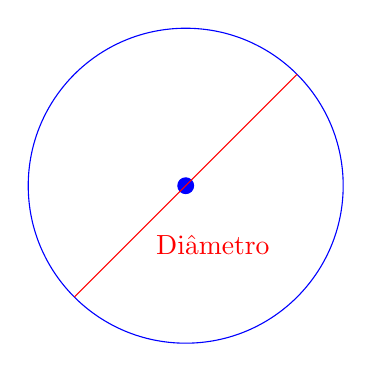
\begin{tikzpicture}
   \draw[color=blue] (0,0) circle(.1)[fill=blue];
   \draw[color=blue] (0,0)  circle(2) (2,0);
   \draw[color=red]
   (-1.414213562373095,-1.414213562373095) --
   (0,0) -- (-0.5,-0.5)node[below right]{Diâmetro} --
   (1.414213562373095,1.414213562373095);
 \end{tikzpicture}
\end{center}

De maneira mais geral, um segmento que une dois pontos na circunferência
é chamado de corda.

\begin{center}
 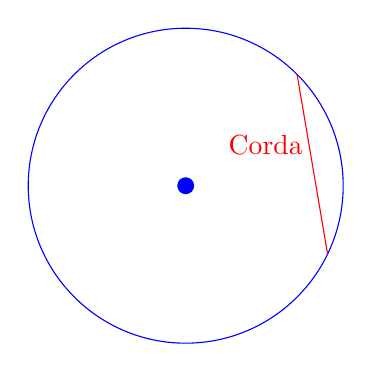
\begin{tikzpicture}
   \draw[color=blue] (0,0) circle(.1)[fill=blue];
   \draw[color=blue] (0,0)  circle(2) (2,0);
   \draw[color=red]
   (1.801937735804838,-0.86776747823511) --
   (1.608075649088966,0.27322304206898)node[above left]{Corda} --
   (1.414213562373095,1.414213562373095);
 \end{tikzpicture}
\end{center}

Uma corda divide a circunferência em duas partes chamadas arcos.

\begin{center}
 \begin{tikzpicture}
   \draw[color=blue] (0,0) circle(.1)[fill=blue];
   \draw[color=blue]
   (1.801937735804838,-0.86776747823511) --
   (1.414213562373095,1.414213562373095);

   \draw[color=red] (1.414213562373095,1.414213562373095)
   arc(45:0:2) node[above right]{Arco}
   arc(0:-25.71428571428571:2);

   \draw[color=orange] (1.414213562373095,1.414213562373095)
   arc(45:200:2) node[below left]{Arco}
   arc(200:334.2857142857143:2);

 \end{tikzpicture}
\end{center}

Para um diâmetro, os dois arcos são chamados semicircunferências.

\begin{center}
 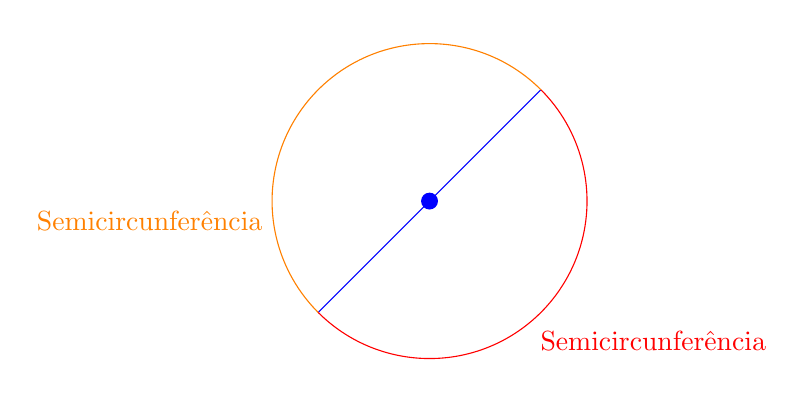
\begin{tikzpicture}
   \draw[color=blue] (0,0) circle(.1)[fill=blue];
   \draw[color=blue]
   (1.414213562373095,1.414213562373095) --
   (-1.414213562373095,-1.414213562373095);

   \draw[color=red] (1.414213562373095,1.414213562373095)
   arc(45:-50:2) node[below right]{Semicircunferência}
   arc(-50:-135:2);

   \draw[color=orange] (1.414213562373095,1.414213562373095)
   arc(45:180:2) node[below left]{Semicircunferência}
   arc(180:225:2);

 \end{tikzpicture}
\end{center}

Uma reta passando por dois pontos de uma circunferência é chamada de secante.
Uma reta que não corta a circunferência é chamada de exterior.
Se corta a circunferência em exatamente um único ponto é chamada de tangente
e é ortogonal ao raio correspondente.

\begin{center}
 \begin{tikzpicture}
   \draw[color=blue] (0,0) circle(.1)[fill=blue];
   \draw[color=blue] (0,0) circle(2) (2,0);
   \draw[color=red] (-2,-2) -- (-1,3) node[above right] {Secante};
   \draw[color=red] (3,-3) -- (5,3) node[above right] {Exterior};

   \begin{scope}[rotate around={-10:(0,0)}]
   \draw[color=blue] (2,0) circle(.1)[fill=blue];
   \draw[color=red] (2,-4) -- (2,4) node[above right] {Tangente};
   \draw[color=orange](1.8,0) -- (1.8,.2) -- (2,.2);
   \draw[color=orange](0,0) -- (2,0);
   \end{scope}

 \end{tikzpicture}
\end{center}

\subsection*{Exercício 1}

Nesse exercício, considere um segmento $[AB]$ e utilizaremos régua e compasso.

\begin{center}
 \begin{tikzpicture}
   \draw[color=blue] (0,0) node[above]{$A$} -- (4,0) node[above]{$B$};
 \end{tikzpicture}
\end{center}

\begin{enumerate}
\item Determine o centro $O$ do círculo de diâmetro $[AB]$, a
circunferência do círculo e um raio $[OC]$ ortogonal a $[AB]$.

\item Indique a semicircunferência associada ao diâmetro $[AB]$ que não contem
  $C$. Trace a corda $BC$ e o menor arco que delimita.
  Compare o comprimento destas circunferências, semicircunferências e arco.

\item Trace a tangente em $C$. O que pode ser dito sobre sua posição relativa a $(AB)$?

\item Trace $D$ simétrico de $A$ com respeito a tangente em $C$.
  De maneira gráfica, encontre a posição relativa a circunferência, para
  a reta $(OD)$, a reta passando por $D$ e paralela a $(OC)$,
  a reta passando por $D$ e paralela a $(AC)$?
\end{enumerate}

\subsection*{Perímetro, área e volume}

O comprimento de uma circunferência é proporcional ao comprimento $2r$ de
seu diâmetro:

$$
L = \pi \times 2r
$$

A constante de proporcionalidade é um número irracional
%%
$$\pi \approx 3.14159265358979323846$$

A área do círculo é
%%
$$
A = \pi \times r^2
$$

Por consequência, se considerarmos um ângulo central de amplitude $\alpha$
($0° \leq \alpha \leq 360°$), o comprimento do arco que correspondente
é
%%
$$
L_{\alpha} = \pi \times 2r \times \frac{\alpha}{360°}
$$
%%
e a área do setor circular que determina é
%%
$$
A_{\alpha} = \pi \times r^2 \times \frac{\alpha}{360°}
$$

A área de um cilindro de altura $h$ e raio $r$ é a soma dos dois círculos
da base ($A = \pi \times r^2$) e da superfície lateral
($L \times h = 2 \pi \times r \times h$. Logo a área do cilindro é
%%
$$A_{h,r} = {2 \pi r^2} + {2\pi r h}$$

O volume do cilindro é
%%
$$V_{h,r} = A_{r} \times h = \pi r^2 h$$

\subsection*{Exercício 2}

Calcule uma aproximação de

\begin{enumerate}
\item A longitude do círculo central de um terreno de futebol (raio de $9.15$m).
\item A área de um disco compacto (diâmetro: $12$cm).
\item O comprimento do arco correspondente a um raio de $R=2$m e ângulo
$\alpha=35$°.
\item A área de um setor correspondente a um raio de $R=3$m e ângulo
$\alpha=75$°.
\item A área de um cilindro de raio $R = 4\text{cm}$ e altura
  $h = 6\text{cm}$.
\end{enumerate}

\subsection*{Exercício 3}

Seja uma pizza de espessura $A = 5$mm e raio $Z = 13$cm.
Utilizando a aproximação $\pi \approx \mathrm{PI} = 3.14$.
O que representa $\mathrm{PI} \times Z \times Z \times A$?
Determine seu valor.

\section{Probabilidade}

\subsection*{Definição}

Wikipédia descreve os conceitos elementares de probabilidade da seguinte
maneira.

A probabilidade é a característica de um evento, que faz com que existam razões
para criar que este se realizará.

A probabilidade $p$ de que ocorra um evento $S$ em um total de $n$ casos
possívels igualmente prováveis é igual a razão entre o número de ocorrências $h$
do evento $S$ (casos favoráveis) e o número total de casos possíveis $n$.

$$
p=P\left(S\right)=\frac {h}{n}
$$

A probabilidade é um número (valor) que varia entre 0 e 1. Quando o evento é
impossível dizemos que sua probabilidade é 0 e se o evento é certo, isso é,
sempre ocorre dizemos que sua probabilidade é 1.

A probabilidade de um evento não ocorrer é dado por $q$, onde:

$$
q=P\left(no \; S\right)=1-\frac {h}{n}
$$

Sabemos que $p$ é a probabilidade de que um evento ocorra e $q$ a probabilidade
de que não ocorra, então $p + q = 1$.

\subsection*{Exemplo}

Quando lançamos uma moeda ao ar, temos $n = 2$ eventos possíveis para o lado da
moeda: ``cara'' ou ``coroa''. Se $S$ é o evento de obtermos ``coroa'', então a
probabilidade de obtermos ``coroa'' é $p = \frac{1}{2}$
e a probabilidade de obtermos ``cara'' é
$q = 1 - p = 1 - \frac{1}{2} = \frac{1}{2}$.
Aqui, supomos que o evento da moeda desaparecer é impossível e portanto sua
probabilidade é $0$.

\subsection*{Exercício 4}

Em um baralho de 52 cartas, qual é a probabilidade de tirarmos:

\begin{enumerate}
  \item Uma carta do naipe de ouro.
  \item Uma carta que é um rei.
  \item Uma carta de paus.
  \item Uma carta que é uma figura (às, rei, dama ou valete).
  \item Um número par.
\end{enumerate}

\subsection*{Regras Aditiva e Multiplicativa}

Se $A$ e $B$ são dois eventos mutuamente exclusivos, temos
%%
$$
P(A \text{ou} B) = P(A) + P(B)
$$

Se $A$ e $B$ são não exclusivos, $P(A \text{e} B) \neq 0$ e 
%%
$$
P(A \text{ou} B) = P(A) + P(B) - P(A \text{e} B)
$$

Se $A$ e $B$ são independentes,
%%
$$
{P(A \text{e} B)} = {P(A)} \times {P(B)}
$$

Se $A$ e $B$ são dependentes, e $P\left(B/A\right)$ é a probabilidade
de $B$ sabendo que $A$ ocorre, temos
%%
$$
{P(A \text{e} B)} = {P(A)} \times {P\left(B/A\right)}
$$

\subsection*{Exemplo}

Considere três bolas de um saco, de cores amarela, branca e azul.
Se $A$ é o evento de tirar a bola amarela, $B$ é de tirar a bola branca
e $C$ de tirar a bola azul.

Se tirarmos uma bola do saco, a probabilidade de tirar a bola amarela ou a bola
branca é
$P(A \text{ou} B) = P(A) + P(B) = \frac{1}{3} + \frac{1}{3}$ por que
$A$ e $B$ são excludentes. Se $\bar{A}$ é a probabilidade de tirarmos a bola
amarela, 
 $\bar{A}$ e $C$ não são mutuamente excludentes porque
$C$ implica $\bar{A}$:
$P(\bar{A} \text{e} C) = P(C) = \frac{1}{3} \neq 0$. Então

$
P(\bar{A} \text{ou} C) = P(\bar{A}) + P(C) - P(\bar{A} \text{e} C)
= \frac{2}{3} + \frac{1}{3} - \frac{1}{3} = \frac{2}{3}
$.

Suponhamos que fizemos esse experimento duas vezes.
Seja $A_1, B_1, C_1$ os eventos do primeiro experimento e
$A_2, B_2, C_2$ os eventos do segundo. $A_1$ e $B_2$ são independentes e
portanto a probabilidade de tirar a bola amarela no primeiro experimento
e a bola branca no segundo experimento é
$P(A_1 \text{y} B_2) = {P(A_1)} \times {P(B_2)} = \frac{1}{3} \frac{1}{3} =
\frac{1}{9}$.

Finalmente, tiramos uma bola (seja $A_1', B_1', C_1'$ os eventos
correspondentes) e se a colocarmos no saco, tiramos uma segunda bola
(seja $A_2', B_2', C_2'$ os eventos correspondentes). A probabilidade de
tirar uma bola amarela e depois uma bola branca é
${P(A_1' \text{y} B_2')} = P(A_1') \times {P(B_2' / A_1')} =
\frac{1}{3} \times \frac{1}{2} = \frac{1}{6}$.

\subsection*{Exercício 5}

Considere um baralho de 52 cartas:

\begin{enumerate}

  \item Tiramos uma carta e, sem voltá-la ao baralho, retiramos uma segunda carta.
  Seja $A$ o evento de ``tirar um rei como primeira carta''
  e $B$ o evento de ``tirar uma figura como segunda carta''.
  Determine $P(A \text{e} B)$.

\item Seja $C$ o evento de ``tirar um rei'' e $B$ o evento de
  ``tirar um número par''. Determine $P(C \text{ou} D)$.

\item Tiramos três cartas (colocamos cada carta de volta ao baralho depois de
  tirá-la).
  Seja $E$ o evento de ``tirar o sete de ouro como primeira carta'',
  $F$ o evento de ``tirar um rei como segunda carta'',
  $G$ o evento de ``tirar uma figura como terceira carta''. Determine
  $P(E \text{e} F \text{e} G)$.

\item Seja $H$ o evento de ``tirar uma carta de paus'' e $I$ o evento de
  ``tirar uma figura''. Determine $P(H \text{e} I)$ e $P(H \text{ou} I)$.

\end{enumerate}

\subsection*{Exercício 6 (Distribuição binomial)}

Realizamos um experimento com uma probabilidade $p$ de sucesso.

\begin{enumerate}
  \item Qual é a probabilidade de fracasso desse experimento?
  \item Se realizamos o experimento duas vezes, qual é a probabilidade
    de termos dois sucessos, dois fracassos, um sucesso e um fracasso?
  \item Realizamos o experimento três vezes. Qual é a probabilidade de
    obtermos um total de dois sucessos se ao final do segundo experimento já temos
    dois sucessos, dois fracassos, um sucesso e um fracasso?
  \item Realizamos o experimento $n$ vezes e consideramos $0 \leq m \leq n$.
    Qual é a probabilidade de obtermos $m$ sucessos se ao final do
    experimento $n-1$ já obtemos $m-1$ sucessos, $m$ sucessos, e em outros
    casos?
  \item Notamos $N! = 1 \times 2 \times \ldots \times N$ e
    $\binom{N}{K} = \frac{N!}{{K!}{(N-K)!}}$. Seja $A_m^n$ a probabilidade
    de obter $m$ sucessos em $n$ experimentos. Nossa conjectura é
    $$
    P(A_m^n) = \binom{n}{m} p^m \left(1-p\right)^{n-m}
    $$
   
    Verifique que a fórmula é correta para $n = 1, 2$. Se é correta para $n - 1$
    experimentos, mostre que também é correta para $n$ experimentos.
  \item Jogamos ``cara'' ou ``coroa'' $10$ vezes. Qual é a probabilidade de
    obtermos 9 sucessos?
  \item Considere o seguinte experimento: tirar uma carta em um baralho e
    obtermos um sucesso de a carta for de copas. Indique as probabilidades $p$ e
    $1 - p$ de sucesso/fracasso. Se realizarmos este experimento $5$ vezes, qual
    é a probabilidade de obtermos $3$ ou mais sucessos?
\end{enumerate}

\section{Solução do Exercícios}

\subsection*{Exercício 1}

\begin{enumerate}
  \item O centro de $O$ é o meio do segmento $[AB]$ então podemos construí-lo
    com a técnica da mediatriz. Depois podemos traçar com o compasso a
    circunferência de raio $OA$. A mediatriz intersecta essa circunferência em
    dois pontos, escolhemos o ponto $C$.

    \begin{center}
 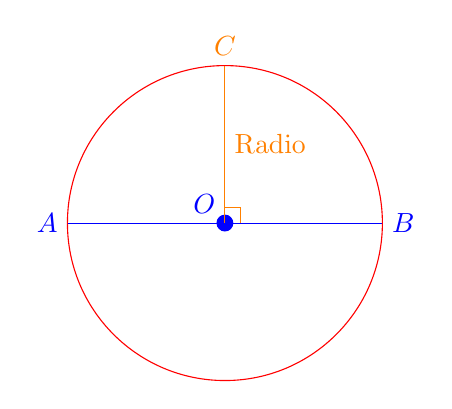
\begin{tikzpicture}
   \draw[color=blue] (-2,0) node[left]{$A$} -- 
   (0,0) node[above left]{$O$} -- (2,0) node[right]{$B$};
   \draw[color=blue] (0,0) circle(.1)[fill=blue];
   \draw[color=red] (0,0) circle(2);
   \draw[color=orange] (0,0) -- (0,1) node[right]{Radio} --
   (0,2) node[above]{$C$} (0,.2) -- (.2,.2) -- (.2,0);
 \end{tikzpicture}
\end{center}
    
    \item O comprimento da semicircunferência é a metade do comprimento da
      circunferência e o comprimento do arco é um quarto do comprimento da
      circunferência.
    \begin{center}
 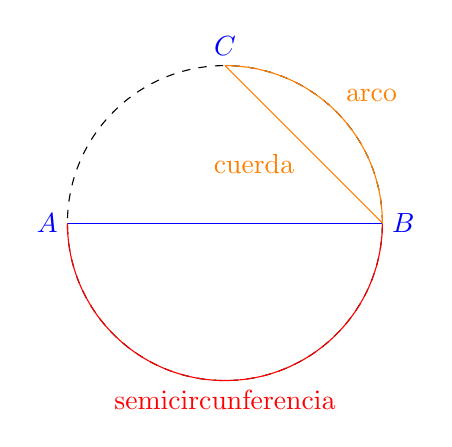
\begin{tikzpicture}
   \draw[dashed] (0,0) circle(2);
   \draw[color=blue] (-2,0) node[left]{$A$} -- (2,0) node[right]{$B$}
   (0,2) node[above]{$C$};
   \draw[color=red] (-2,0) arc(180:270:2) node[below]{semicircunferencia}
   arc(270:360:2);

   \draw[color=orange] (0,2) -- (1,1) node[below left]{cuerda}
   -- (2,0) arc(0:45:2) node[above right]{arco}  arc(45:90:2);
    \end{tikzpicture}
\end{center}

 \item Para traçar a tangente, utilizamos a técnica para construir
   uma reta ortogonal a $(OC)$ e passando pelo ponto $C$.
   Porque $(AC)$ é ortogonal a $(OC)$ e
   $C \notin (AB)$ a tangente é paralela a $(AB)$.

    \begin{center}
    \begin{tikzpicture}
   \draw[color=blue] (-2,0) node[left]{$A$} -- 
   (0,0) node[above left]{$O$} -- (2,0) node[right]{$B$} (0,2) node[above]{$C$};
   \draw[color=blue] (0,0) circle(.1)[fill=blue];
   \draw[color=red] (0,0) circle(2);
   \draw[color=orange] (0,0) --
   (0,2) (0,.2) -- (.2,.2) -- (.2,0);
   \draw[color=green] (-4,2) --
   (2,2) node[above]{Tangente} -- (4,2);

    \end{tikzpicture}
\end{center}

\item São, respectivamente, secante, tangente e exterior à circunferência.

    \begin{center}
    \begin{tikzpicture}
   \draw[color=blue] (-2,0) node[left]{$A$} -- 
   (0,0) node[above left]{$O$} -- (2,0) node[right]{$B$} (0,2) node[above]{$C$};
   \draw[color=blue] (0,0) circle(.1)[fill=blue];
   \draw[color=red] (0,0) circle(2);
   \draw[color=orange] (0,0) --
   (0,2) (0,.2) -- (.2,.2) -- (.2,0);
   \draw[dashed] (-4,2) -- (4,2);
   \draw[color=blue] (-2,4) node[right]{$D$} circle(.1)[fill=blue];

   \draw[color=green] (-3,6) -- (1,-2);
   \draw[color=green] (-2,6) -- (-2,-2);
   \draw[color=green] (0,6) -- (-6,0);
    \end{tikzpicture}
\end{center}

\end{enumerate}

\subsection*{Exercício 2}

\begin{enumerate}
\item $2 \times \pi \times 9.15 \approx 57.5$m.
\item $\pi \times 6^2 \approx 113 \text{cm}^2$.
\item $2 \times \pi \times 2 \times \frac{35}{360} \approx 1.22$m.
\item $\pi \times 3^2 \frac{75}{360} \approx 5.89 \text{m}^2$.
\item ${2 \times \pi \times 4^2} + {2 \times \pi \times 4 \times 6} =
  80\pi \approx 251.33 \text{cm}^2$
\end{enumerate}

\subsection*{Exercício 3}

$\mathrm{PI} \times Z \times Z \times A$ é uma aproximação do volume da pizza.
Obtemos
$3.14 \times 0.5 \times 13 = 20.41 \text{cm}^3$.

\subsection*{Exercício 4}

Existem 52 eventos equiprováveis correspondente a cada carta.

\begin{enumerate}
\item $\frac{1}{52}$ (um sete de ouros)
\item $\frac{4}{52} = \frac{1}{13}$ (4 reis)
\item $\frac{9 + 4}{52} = \frac{1}{4}$ (9 números de paus e 4 figuras de naipes
  diferentes)
\item $\frac{4 \times 4}{52} = \frac{4}{13}$ (4 figuras de 4 paus)
\item $\frac{4 \times 5}{52} = \frac{5}{13}$ (números 2, 4, 6, 8 e 10 de 4
  naipes)
\end{enumerate}

\subsection*{Exercício 5}

\begin{enumerate}

\item No exercício 4, encontramos $P(A) = \frac{1}{13}$
  e $P(\text{tirar uma figura}) = \frac{16}{52}$. Aqui,
  $P(B / A) = \frac{16 - 1}{52 - 1}$ porque existe uma figura/carta a menos
  quando $A$ ocorre. Então
  $P(A \text{e} B) = P(A) \times P(B / A) = 
  \frac{1}{13} \frac{15}{51} = \frac{5}{221}$.

\item No exercício 4, encontramos $P(C) = \frac{1}{13}$ e
  $P(D) = \frac{5}{13}$. Os dois eventos são mutuamente excludentes então
  $P(C \text{ou} D) = \frac{1}{13} + \frac{5}{13} = \frac{6}{13}$.

\item Os três eventos são independentes, então
  $P(E \text{e} F \text{e} G) = {P(E)} \times {P(F)} \times {P(G)}$.
  No exercício 4, encontramos
  $P(E) = \frac{1}{52}$, $P(F) = \frac{1}{13}$ e $P(G) = \frac{4}{13}$.
  Finalmente, $P(E \text{e} F \text{e} G) = \frac{1}{2197}$.

\item No exercício 4, encontramos
  $P(H) = \frac{1}{4}$ e $P(I) = \frac{4}{13}$.
  $H \text{e} I$ é o evento de ``tirar uma figura de paus''. Temos $4$ figuras
  de paus (às, rei, dama e valete) então
  $P(H \text{e} I) = \frac{4}{52}=\frac{1}{13} = P(H) P(I)$ (em particular
  $H$ e $I$ são independentes).
  $P(H \text{uo} I) = P(H) + P(I) - P(H \text{e} I) =
  \frac{1}{4} + \frac{4}{13} - \frac{1}{13} = \frac{25}{52}$.
\end{enumerate}

\subsection*{Exercício 6 (Distribuição Binomial)}

\begin{enumerate}
  \item $1-p$
  \item A probabilidade de obtermos dois sucesso é $p \times p = p^2$.
    A probabilidade de obtermos dois fracassos é ${(1-p)} \times {(1-p)}
    = {(1-p)}^2$. A probabilidade de obtermos um sucesso e um fracasso
    é $1 - p^2 - {(1-p)}^2$. É também a probabilidade do evento
    ``sucesso seguido de um fracasso seguido de um sucesso'' que vale
    $2 p{(1-p)}$.
  \item Se já obtemos $2$ sucessos, precisamos de um fracasso no terceiro
    experimento, o que ocorre com uma probabilidade de $1 - p$.
    Se tivemos $0$ sucessos, é impossível obter um total de $2$ sucessos com o
    último experimento.
    Se tivemos $1$ sucesso, necessitamos de um sucesso no terceiro experimento,
    o que ocorre com uma probabilidade $p$.
  \item Da mesma maneira, é impossível obter $m$ sucessos exceto
    se já tivemos $m-1$ ou $m$ sucessos. Isso ocorre, respectivamente,
    com probabilidade $p$ e $1-p$.

  \item 
    Para $n=1$, temos
    $P(A_0^1) = \binom{1}{0} p^0 \left(1-p\right)^{1-0} = 1-p$
    $P(A_1^1) = \binom{1}{1} p^1 \left(1-p\right)^{1-1} = p$.
    Para $n=2$, temos
    $P(A_0^2) = \binom{2}{0} p^0 \left(1-p\right)^{2-0} = \left(1-p\right)^2$
    $P(A_2^2) = \binom{2}{2} p^2 \left(1-p\right)^{2-2} = p^2$ y
    $P(A_1^2) = \binom{2}{1} p^1 \left(1-p\right)^{2-1} = 2 p \left(1-p\right)$.
    Pela pergunta anterior,
%%
    $$
    P(A_m^n) = P(A_{m-1}^{n-1}) P(A_m^n / A_{m-1}^{n-1}) +
    P(A_{m}^{n-1}) P(A_m^n / A_{m}^{n-1}) =
    p {P(A_{m-1}^{n-1})} + \left(1-p\right) {P(A_{m}^{n-1})}
    $$

    Se supormos que nossa conjectura é correta para
    ${P(A_{m-1}^{n-1})}$
    e ${P(A_{m}^{n-1})}$, obtemos
%%
    $$
    P(A_m^n) = \left( 
    \binom{n-1}{m-1} + \binom{n -1}{m}
    \right) p^m \left(1-p\right)^{n-m}
    $$

    Mas
    $\binom{n-1}{m-1} + \binom{n -1}{m}  = 
    \frac{\left(n-1\right)!}{\left(n-m\right)! m!} 
    \left(m + \left(n-m\right)\right) = \binom{n}{m}$

  \item A probabilidade para um jogo é $p = \frac{1}{2}$.
    Então
    $P(A_{10}^{10}) = \binom{10}{9} \left(\frac{1}{2}\right)^{9} 
    \left(\frac{1}{2}\right)^{10-9} = \frac{10}{2^{10}} = \frac{5}{512}
    = 0.009765625$

  \item $p = \frac{1}{4}$ e $1-p = \frac{3}{4}$.
    A probabilidade de obtermos $3$ ou mais sucessos é
    $P(A_{3}^{5}) + P(A_{4}^{5}) + P(A_{5}^{5}) =
    \frac{53}{512} = 0.103515625$.
\end{enumerate}
